\chapter{Технологическая часть}

\section{Средства реализации}

Для реализации программного обеспечения был выбран язык C++~\cite{iso_cpp_2020}. Выбор C++ обусловлен наличием всех необходимых компонентов в стандартной библиотеке для реализации алгоритмов, разработанных в результате проектирования. В частности, были использованы следующие компоненты:
\begin{itemize}
    \item контейнер \texttt{std::vector} для хранения вершин, нормалей, треугольников и листьев сцены;
    \item строки \texttt{std::string} и алгоритмы работы с ними --- для представления и итеративного расширения последовательности символов L-системы;
    \item \texttt{std::stack} --- для реализации состояния черепашьей-интерпретации (сохранение и восстановление позиции и ориентации при обходе ветвей);
    \item средства генерации псевдослучайных чисел (\texttt{std::default\_random\_engine} и \texttt{std::uniform\_real\_distribution}) --- для внесения естественной вариативности в углы ветвления и длины сегментов;
    \item математические функции стандартной библиотеки (<cmath>).
\end{itemize}

В качестве сторонней библиотеки для реализации графического пользовательского интерфейса был выбран фреймворк Qt~\cite{qt}. Выбор обусловлен его кроссплатформенностью, нативной поддержкой языка C++ и наличием визуального редактора интерфейсов (Qt Designer)~\cite{qtdesigner}.

В качестве системы управления процессом сборки был выбран CMake~\cite{cmake}. СMake представляет собой кроссплатформенную систему автоматизации сборки, которая генерирует файлы конфигурации для различных
систем сборки.

В качестве среды разработки использовался CLion~\cite{clion}, обеспечивающий все необходимые
инструменты для работы с проектами на C++.

\section{Структура программы}

Программа построена по объектно-ориентированному принципу и состоит из нескольких взаимосвязанных модулей, каждый из которых отвечает за определённую функциональную область.

Модуль генерации геометрии отвечает за синтез структуры дерева и построение полигональной модели.
Содержит:
\begin{itemize}
\item \texttt{LSystemGenerator} --- реализует итеративную подстановку правил L-системы и возвращает строку команд;
\item \texttt{TurtleInterpreter3D} --- интерпретирует строку команд с помощью трёхмерной черепашьей графики и генерирует полигональную сетку ствола и ветвей, а также позиции листьев.
\end{itemize}

Модуль представления сцены определяет структуру виртуального мира и объектов в нём.
Содержит:
\begin{itemize}
\item \texttt{Scene} --- контейнер, хранящий все объекты сцены, источник света и камеру;
\item \texttt{SceneObject} --- абстрактный базовый класс для всех объектов сцены;
\item \texttt{MeshObject} --- объект сцены, содержащий одну полигональную сетку (используется для ствола и ветвей);
\item \texttt{InstancedMeshObject} --- объект для эффективного отображения множества копий одной геометрии (листья).
\end{itemize}

Модуль рендеринга осуществляет программную визуализацию сцены.
Содержит:
\begin{itemize}
\item \texttt{Rasterizer} --- основной класс растеризатора, выполняющий отрисовку треугольников с учётом z-буфера, освещения и теней;
\item \texttt{ShadowMapRenderer} --- специализированный рендерер для генерации карты теней;
\item \texttt{BaseVisitor} --- абстрактный класс, реализующий паттерн <<Посетитель>>.
\item \texttt{DrawVisitor}, \texttt{ShadowVisitor} --- реализуют паттерн <<Посетитель>> для обхода объектов сцены с разными целями (основной рендеринг/теневой проход).
\end{itemize}

Модуль управления освещением выполняет расчёт цвета фрагментов на основе выбранной модели.
Содержит:
\begin{itemize}
\item \texttt{Lighting} --- статический класс с методом \texttt{calculatePhong} для расчёта освещения по модели Блинна–Фонга.
\end{itemize}

Модуль пользовательского интерфейса обеспечивает взаимодействие пользователя с системой.
Содержит:
\begin{itemize}
\item \texttt{MainWindow} --- главное окно приложения на основе Qt, содержащее элементы управления (поля ввода, слайдеры) и виджет отображения;
\item \texttt{SceneRenderer} --- связующий компонент, координирующий генерацию, настройку камеры, источников света и вызов рендеринга.
\end{itemize}

К вспомогательным компонентам относятся:
\begin{itemize}
\item \texttt{Camera}, \texttt{OrbitCamera}, \texttt{FreeCamera} — управление точкой зрения;
\item \texttt{Mesh}, \texttt{Vertex}, \texttt{Triangle} — представление геометрии;
\item \texttt{Light}, \texttt{Material} — параметры освещения и материалов.
\end{itemize}

Взаимодействие модулей осуществляется через чётко определённые интерфейсы:
\begin{itemize}
    \item модуль генерации выдаёт \texttt{Mesh} и позиции листьев;
    \item модуль сцены инкапсулирует данные;
    \item модуль рендеринга принимает сцену, возвращает изображение;
    \item интерфейс инициирует генерацию и отображает результат.
\end{itemize}

На рисунке~\ref{fig:uml} показана диаграмма классов программы.
\begin{figure}[H]
    \centering
    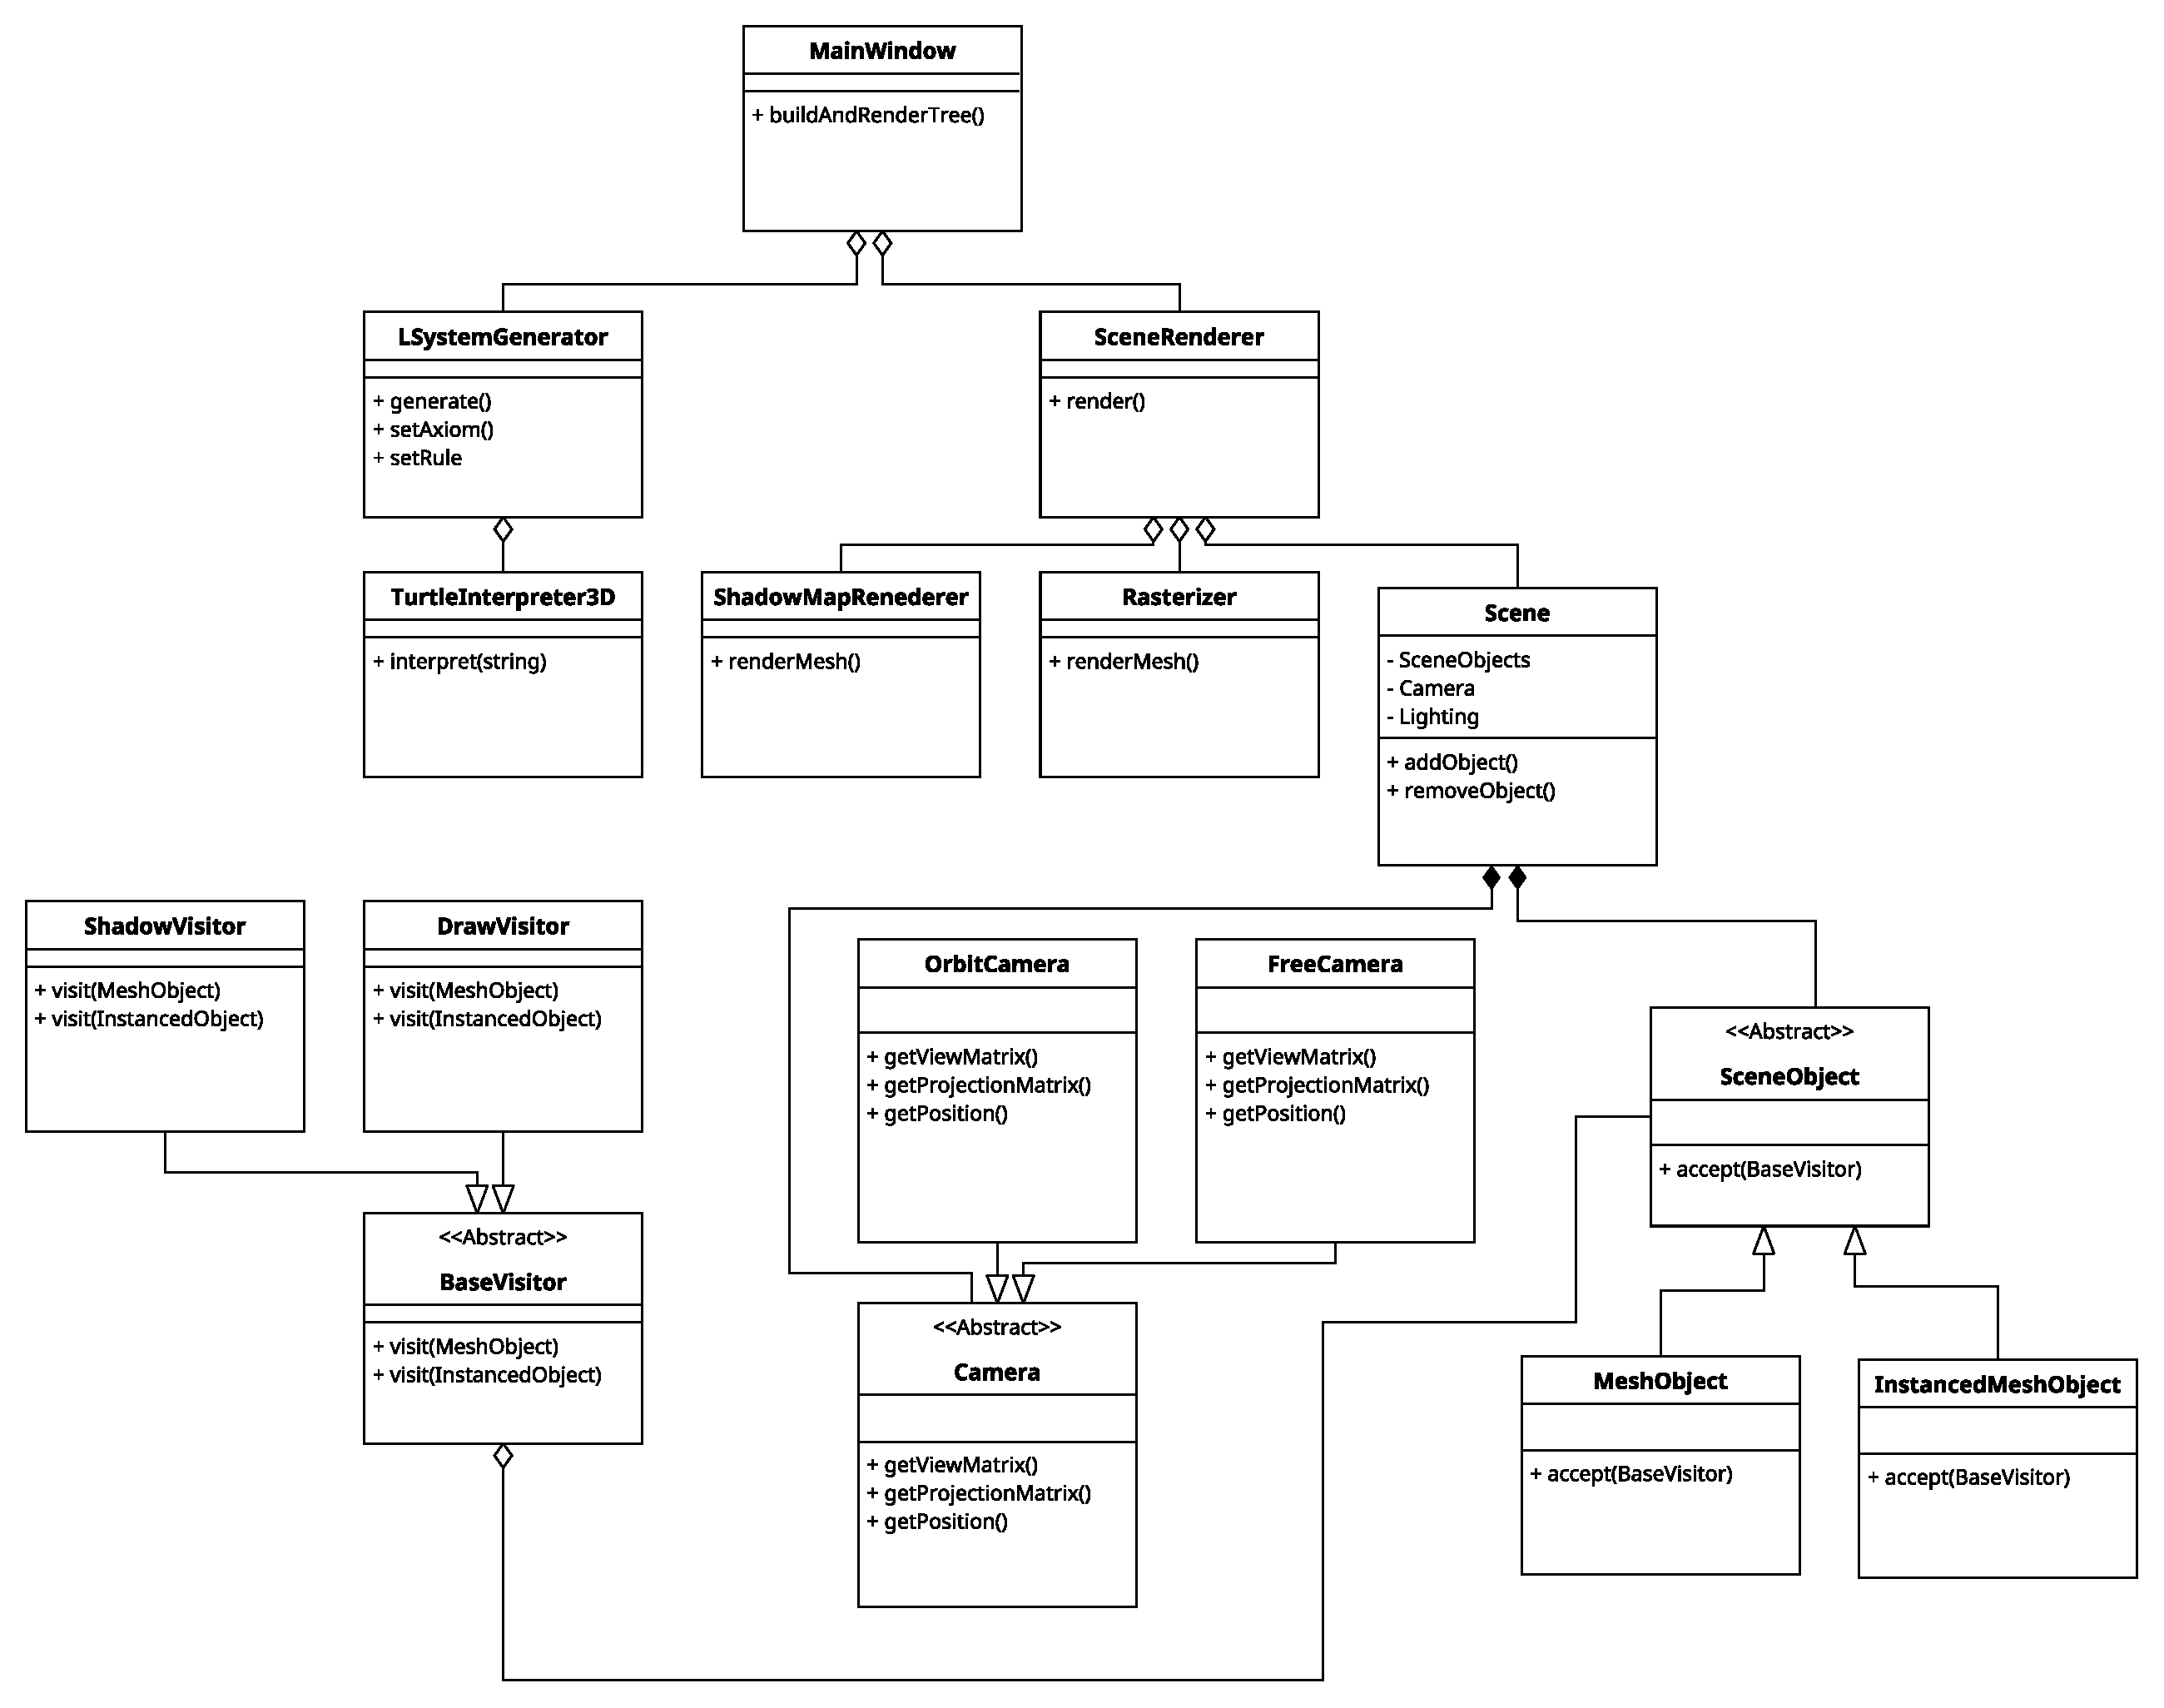
\includegraphics[width=\textwidth]{images/uml.pdf}
    \caption{UML-диаграмма классов программы}
    \label{fig:uml}
\end{figure}

\section{Реализация алгоритмов}
В листинге~\ref{lst:z-buffer} приведена реализация алгоритма растеризации с учётом буфера глубины.

В листинге~\ref{lst:shadow-map} приведена реализация алгоритма построения карты теней.

В листинге~\ref{lst:phong} приведена реализация модели освещения по Блинну-Фонгу.

В листинге~\ref{lst:lsys} приведена реализация алгоритма построения структуры дерева.

\section{Описание пользовательского интерфейса}
Пользовательский интерфейс состоит из панели управления параметрами и области визуализации трёхмерной сцены.

\subsection{Структура интерфейса}

Главное окно приложения разделено на две области:
\begin{itemize}
    \item левая панель управления с элементами настройки параметров генерации;
    \item правая область визуализации с отображением трёхмерной модели дерева.
\end{itemize}

Панель управления организована в виде групповых элементов, каждый из которых отвечает за определённую категорию параметров.

\subsection{Основные элементы управления}

Группа <<Готовые деревья>> содержит выпадающий список с предустановленными конфигурациями деревьев различных типов.

Группа <<Параметры L-системы>> включает:
\begin{itemize}
    \item поле ввода аксиомы L-системы;
    \item таблицу правил подстановки с возможностью добавления и редактирования;
    \item выпадающий список символов (A--Z) для выбора символа правила;
    \item поля настройки количества итераций, угла поворота и длины шага.
\end{itemize}

Система поддерживает стандартные операторы L-системы: F/G (рисование), f (перемещение), +/- (повороты), \&/\^{} (наклоны), [ ] (ветвление), L (листья).

Группа <<Геометрия дерева>> содержит параметры:
\begin{itemize}
    \item базовый радиус ствола (0,01--2,0);
    \item коэффициент уменьшения радиуса ветвей (0,1--0,99);
    \item минимальный радиус конечных ветвей (0,001--0,1);
    \item фактор гравитации для провисания ветвей (0,0--0,5);
    \item количество сегментов в поперечном сечении (3--20).
\end{itemize}

Группа <<Параметры освещения>> позволяет настроить интенсивность и направление источника света (координаты x, y, z).

Группа <<Камеры>> предоставляет выбор между орбитальной камерой (вращение вокруг объекта) и свободной камерой (перемещение в пространстве).

Группа <<Тени>> содержит переключатель для включения/отключения расчёта теней методом shadow mapping.

\subsection{Управление и визуализация}

Генерация дерева выполняется по нажатию кнопки <<Сгенерировать дерево>>.

Управление камерой осуществляется с помощью мыши (перетаскивание, колесо прокрутки) и клавиатуры (W/A/S/D для перемещения, Q/E для вертикального движения, 1/2/3 для предустановленных ракурсов).

Область визуализации отображает результат рендеринга. Размер области автоматически адаптируется при изменении размера окна.

\section{Демонстрация работы программы}
На рисунках~\ref{fig:exmp1} и~\ref{fig:exmp2} представлены примеры работы программы.

\begin{figure}[H]
    \centering
    \includegraphics[width=\textwidth]{images/example.png}
    \caption{Пример работы программы для дерева с листьями}
    \label{fig:exmp1}
\end{figure}

\begin{figure}[H]
    \centering
    \includegraphics[width=\textwidth]{images/example2.png}
    \caption{Пример работы программы для дерева без листьев}
    \label{fig:exmp2}
\end{figure}

\section{Вывод}
В технологической части были описаны средства реализации программного обеспечения, описана его структура, и была приведена демонстрация работы программы.